% LaTeX source for ``Algorithms for Computer Simulation of Molecular Systems''
% Copyright (c) 2023 รังสิมันต์ เกษแก้ว (Rangsiman Ketkaew).

% License: Creative Commons Attribution-NonCommercial-NoDerivatives 4.0 International (CC BY-NC-ND 4.0)
% https://creativecommons.org/licenses/by-nc-nd/4.0/

{
% \pagenumbering{gobble}

\chapter*{\centering สิ่งที่ควรทราบเกี่ยวกับหนังสือเล่มนี้}
\addcontentsline{toc}{chapter}{สิ่งที่ควรทราบเกี่ยวกับหนังสือเล่มนี้}

หนังสือเล่มนี้มีหนังสือต่างประเทศหลายเล่มเป็นแหล่งข้อมูลอ้างอิงทางวิชาการเพื่อให้มั่นใจได้ว่าความรู้ที่ผู้อ่านจะได้ศึกษาจากหนังสือเล่มนี้นั้นถูกต้อง
อย่างไรก็ตามผมไม่สามารถการันตีได้ 100 เปอร์เซ็นต์ว่าหนังสือเล่มนี้ไม่มีข้อผิดพลาดเลยแม้แต่จุดเดียว ข้อผิดพลาดเล็กน้อยอาจจะเกิดจากการพิมพ์ผิด 
เป็นต้น ส่วนข้อผิดพลาดทางเนื้อหานั้นผมค่อนข้างมั่นใจว่ามีน้อยมากเพราะว่าผมได้ใช้หนังสือได้ที่รับการยอมรับและความนิยมในกลุ่มนักวิจัยทางด้าน 
Quantum Chemistry, Electronic Structure และ \textit{Ab Initio} Molecular Dynamics หลาย ๆ เล่มมาเป็นหนังสืออ้างอิง 
รวมถึงได้พูดคุยและสอบถามกับนักวิจัยด้านเคมีควอนตัมคนอื่น ๆ ทั้งที่เป็นเพื่อนรวมงานและคนที่ผมได้ไปพบเจอตามงานประชุมวิชาการ 
จึงทำให้มั่นใจได้ว่าความรู้ที่ถ่ายทอดผ่านหนังสือเล่มนี้นั้นถูกต้อง สำหรับสไตล์การใช้ภาษาในการเขียนหนังสือเล่มนี้ไม่วิชาการมากเกินไป 
ซึ่งผมพยายามเลือกใช้คำง่าย ๆ ให้มากที่สุด แต่ถึงอย่างนั้นก็ตามผมก็ไม่อาจที่จะหลีกเลี่ยงการใช้คำศัพท์เชิงเทคนิคได้

หนังสือ 6 เล่มที่ผมคิดว่าเขียนได้ดีมาก ๆ และผมใช้เป็นหนังสืออ้างอิงไม่เพียงแค่สำหรับเขียนหนังสือเล่มนี้แต่ยังใช้ในการทำงานวิจัยของผมเองด้วยมีดังนี้

\begin{figure}[H]
    \begin{center}
        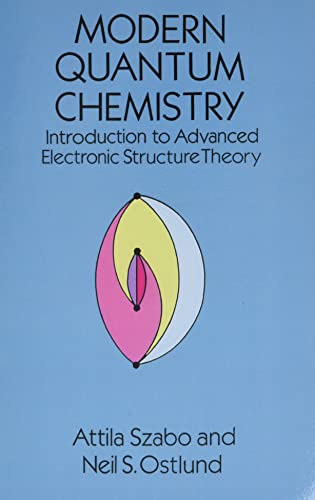
\includegraphics[height=6cm]{fig/modern-qm.jpg} 
        \hspace{0.5em}
        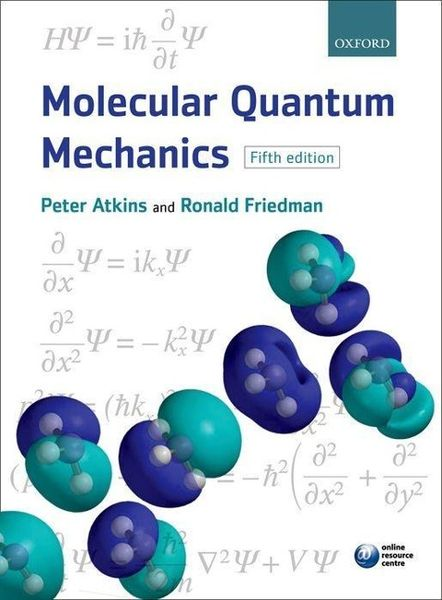
\includegraphics[height=6cm]{fig/mol-quan-mech.jpeg} 
        \hspace{0.5em}
        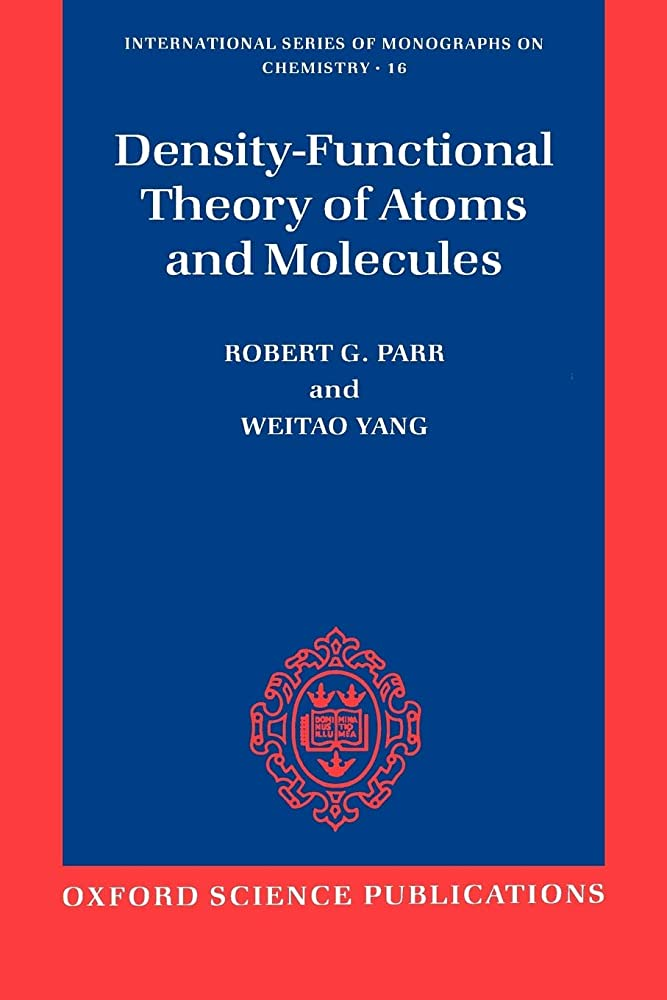
\includegraphics[height=6cm]{fig/dft-atom-mol.jpg} \\
        \vspace{1em}
        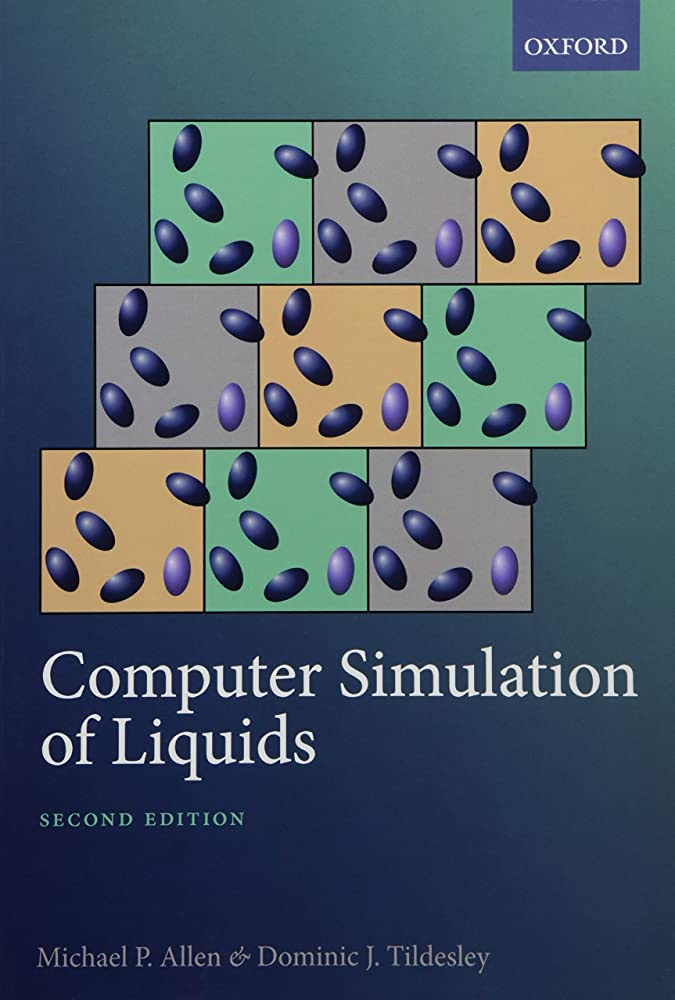
\includegraphics[height=6cm]{fig/com-sim-liq.jpg} 
        \hspace{0.5em}
        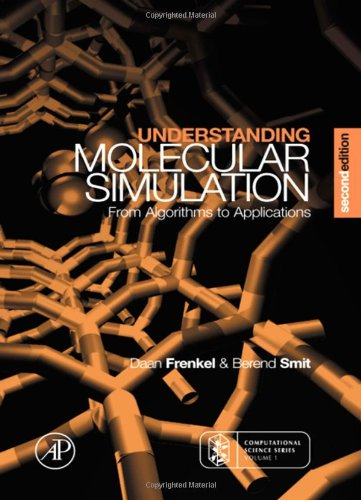
\includegraphics[height=6cm]{fig/understand-mol-sim.jpg}
        \hspace{0.5em}
        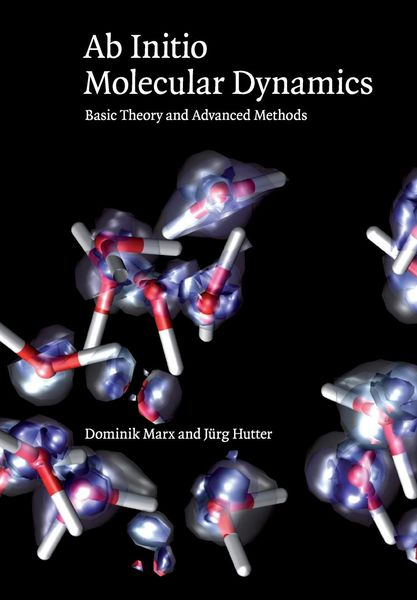
\includegraphics[height=6cm]{fig/aimd.jpeg}
    \end{center}
\end{figure}

\begin{enumerate}[topsep=0pt,noitemsep]
    \setlength\itemsep{1em}
    \item Modern Quantum Chemistry: Introduction to Advanced Electronic Structure Theory
    แต่งโดย Attila Szabo และ Neil S. Ostlund\autocite{szabo1996}

    \item Molecular Quantum Mechanics (5th Edition)
    แต่งโดย Peter W. Atkins และ Ronald S. Friedman\autocite{atkins2010}

    \item Density-Functional Theory of Atoms and Molecules 
    แต่งโดย Robert G. Parr และ Yang Weitao\autocite{parr1994}

    \item Computer Simulation of Liquids (2nd Edition)
    แต่งโดย Michael P. Allen และ Dominic J. Tildesley\autocite{allen2017}
    
    \item Understanding Molecular Simulation: From Algorithms to Applications (2nd Edition)
    แต่งโดย Daan Frenkel และ Berend Smit\autocite{frenkel2001}

    \item \textit{Ab Initio} Molecular Dynamics: Basic Theory and Advanced Methods
    แต่งโดย Dominik Marx และ Juerg Hutter\autocite{marx2009}
    
\end{enumerate}

หนังสือเล่มนี้\underline{เหมาะ}สำหรับนักศึกษา นักวิจัย ผู้ที่สนใจในสาขาเคมีทฤษฎีและเคมีคำนวณและผ่านการเรียนวิชาเคมีเชิงฟิสิกส์มาแล้ว 
โดยเนื้อหาในหนังสือเล่มนี้เน้นไปที่การอธิบายทฤษฎีและพิสูจน์ที่มาของสมการทางกลศาสตร์ควอนตัมและโครงสร้างเชิงอิเล็กทรอนิกส์ของอะตอมและโมเลกุล%
รวมถึงแบบจำลองของระบบโมเลกุล นอกจากนี้ยังอธิบายการประยุกต์ใช้อัลกอริทึมทางคอมพิวเตอร์สำหรับการเขียนโปรแกรมคำนวณและการประมวลผล%
บนคอมพิวเตอร์สมรรถนะสูงอีกด้วย

หนังสือเล่มนี้\underline{ไม่เหมาะ}สำหรับผู้ที่ยังไม่เคยเรียนวิชาเคมีเชิงฟิสิกส์หรือเคมีควอนตัมมาก่อนเพราะว่าอาจจะตกใจกับคำศัพท์ทางเทคนิคและ%
สมการต่าง ๆ ได้ อย่างไรก็ตามถ้าหากผู้อ่านสามารถทำความเข้าใจเนื้อหาของหนังสือเล่มนี้ได้โดยที่ยังไม่เคยศึกษาเคมีควอนตัมมาก่อนเลยก็ถือว่าเยี่ยมมาก ๆ 
นอกจากนี้แล้วในการทำความเข้าใจเนื้อหาในหนังสือเล่มนี้นั้นจะต้องอาศัยความรู้ทางคณิตศาสตร์พีชคณิตเยอะมาก ๆ โดยเฉพาะความรู้เกี่ยวกับเวกเตอร์ 
เมทริกซ์ แคลคูลัส รวมไปถึงเทคนิคต่าง ๆ ทางคณิตศาสตร์ เช่น Optimization, Decomposition, และ Diagonalization ดังนั้นผู้อ่านควร%
จะต้องมีความรู้คณิคศาสตร์เหล่านี้มาบ้างแล้ว

คำแนะนำในการศึกษาทฤษฎีทางเคมีควอนตัมจากประสบการณ์ส่วนตัวของผมที่อยากจะแบ่งปันมี 3 ข้อคือ 

\begin{enumerate}[topsep=0pt,noitemsep]
    \setlength\itemsep{1em}
    \item อ่านตำรา (Textbook) ทีละเล่ม : สำหรับผู้ที่เริ่มต้นนั้นควรเลือกหนังสือเพียงเล่มเดียว ถ้าหากว่าอ่านหลายเล่มพร้อม ๆ 
    กันแล้วสลับอ่านไปมาก็อาจจะทำให้เกิดความสับสนได้เพราะว่าหนังสือแต่ละเล่มนั้นจะมีการใช้สัญลักษณ์หรือคำศัพท์เฉพาะทางที่ต่างกันได้
    
    \item อ่านบทความวิชาการเพื่ออัพเดทความรู้ : ปฏิเสธไม่ได้เลยว่าการทำวิจัยในปัจจุบันนั้นดำเนินไปอย่างรวดเร็วมาก ๆ เนื่องจากว่าเรามี%
    คอมพิวเตอร์ที่มีประสิทธิภาพมากขึ้น รวมถึงกระบวนการตีพิมพ์งานวิชาการนั้นก็ไม่ได้ช้าเหมือนในอดีต ดังนั้นการอ่านบทความวิชาการ เช่น 
    บทความวิจัย, บทความรีวิว รวมถึงสรุปข่าวต่าง ๆ จึงมีความสำคัญอย่างมากเพราะว่าเราจะได้อัพเดทความรู้ของเราตลอดเวลา

    \item การเขียนโปรแกรม : การเขียนโปรแกรมนั้นจะมีลำดับขั้นตอนที่ชัดเจน ตรงไปตรงมา และไม่สามารถข้ามขั้นตอนได้ ถ้าหากว่าเราศึกษา%
    การเขียนโปรแกรมควบคู่ไปกับการทฤษฎีที่สนใจก็จะทำให้เราเข้าใจที่มาที่ไปได้ง่ายขึ้น
\end{enumerate}

}
